% Licensed to the Apache Software Foundation (ASF) under one or more
% contributor license agreements. See the NOTICE file distributed with
% this work for additional information regarding copyright ownership.
% The ASF licenses this file to You under the Apache License, Version 2.0
% (the ``License''); you may not use this file except in compliance with
% the License. You may obtain a copy of the License at
%
% http://www.apache.org/licenses/LICENSE-2.0
%
% Unless required by applicable law or agreed to in writing, software
% distributed under the License is distributed on an ``AS IS'' BASIS,
% WITHOUT WARRANTIES OR CONDITIONS OF ANY KIND, either express or implied.
% See the License for the specific language governing permissions and
% limitations under the License.

\subsubsection{Configuring a Share Connection}

You must fill in the following tabs if you are configuring a Share
connection:

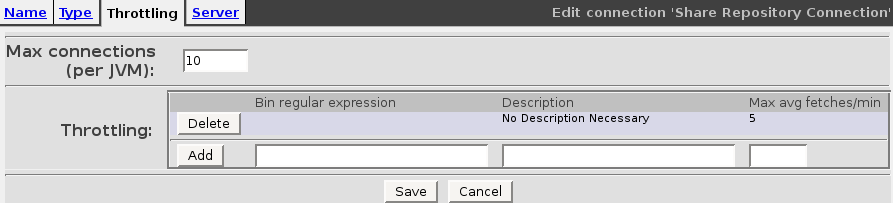
\includegraphics[width=300pt]{Share-edit-repository-tab3}

\begin{itemize}

\item \textbf{Max connections (per JVM):} Here you can set the maximum
number of connections to your repository.  \ifCombinedConnectorGuide
The maximum number of connections per JVM is important for three
reasons; licensing, appliance resources, and the possiblity of
overwhelming the ingestion interface. For a more complete explanation,
see the Max Connections item on page \pageref{maxrepocon}.\fi

\ifShareGuide
The maximum number of connections per JVM is important for three reasons.
First, the number of connections may impact the licensing on your document
server, depending on the repository.

Second, the number of connections may impact the resources
available on the appliance. If the connector framework is slowing down
your appliance, lowering this number should help.

Third, only ten document streams can be processed by the appliance
at one time.  If you are also using other repository connectors or
the \command{ingest} command on the appliance, you should reduce this
number to prevent contention for the Ingestion interface. The Share
Connector will never overwhelm the interface on its own, but when other
applications are also using the ingestion interface, it may be best to
set the number of repository connections to five or even fewer.
\fi

\item \textbf{Throttling:} Here you can set a maximum document fetch
rate for the repository connection.


The maximum fetch rate allows you to set three things: Expression,
description, and fetches per minute. Expression allows you to provide
a regular expression to match against document bins.  Each document
ingested through a connector is associated with one or more document
bins. These bins represent the servers that the connector interacts
with to obtain the document.  Typically, a document will be associated
with only one document bin, representing the repository server hosting
the document. For some repository connections, documents ingested
through the connector can be hosted by different servers. In the Share
Connector, documents only come from one server, which you will set on
the following tab. Simply leave the expression blank; this will match
any server you enter on the following tab.  All you need to set is the
number of document fetches per minute.  Description is an optional
field that allows you to provide a short text description of the
throttle.  Once you have set the fetch rate and optional description,
click Add.




\end{itemize}

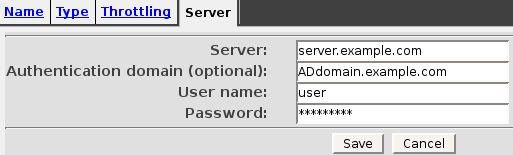
\includegraphics[width=300pt]{Share-edit-repository-tab4}

\begin{itemize}

\item \textbf{Server:} The fully qualified sever name of network share
with which you wish to connect.

\item \textbf{Authentication domain (optional):} The Active Directory
domain that your network share is a part of. This is an optional
argument. 

\item \textbf{User name:} The user name that the GTS appliance will
use to connect to the network share for this repository connection.
Typically, your network share administrator will create this account
specifically for use by the appliance. The account used by the GTS
appliance must have sufficient authority to retrieve files and their
corresponding ACLs.

\item \textbf{Password:} The password corresponding to the
user name given to the GTS.

The Active Directory domain should only be included once between the
``Authentication domain'' and ``User name'' fields, but may not be
necessary for either. The exact phrasing required by the crawler
depends on the configuration of your network share. This is a common
cause of a failed repository connection. In order to correctly
configure your repository connection you may need to try all 3
possible pairings: \command{ADdomain.example.com} with \command{user}, a
blank domain with \command{user@ADdomain.example.com}, and a blank
domain with \command{user}.

\end{itemize}

\note{The Share Connector gets its domain authentication information by
querying the relevant AD domain for a list of domain controllers and
then trying the first domain controller on that list. If your domain
controllers are inaccessible, the Share Connector will not be able to
function.} 

% This should go in a Troubleshooting section when we have one,
% but rc4 is not the time.

After entering this information, you will be taken to the repository 
connection status page for this repository:

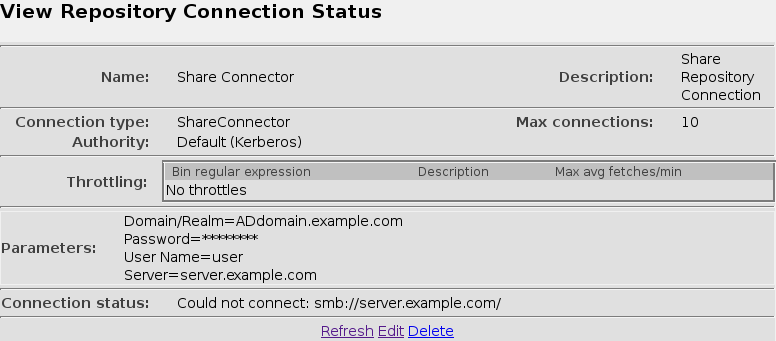
\includegraphics[width=300pt]{Share-view-repo-conn-status}

In this example (which does not contain accurate information for any
Share Connector), the Connection Status is ``Connection failed.''  If
you see this message, you most likely have incorrectly entered one of
the fields, and should click ``Edit'' to fix the data. If you have
entered everything as you intended, please inform your network share
administrator; you may not have been given the correct information.
